\section{Motivation for Scalable QoE Annotation} \label{MOTIVATION}

In this section, we describe the need for new QoE metrics for enterprise networks and the limitations of existing work. 

\noindent {\bf Lack of QoE information from applications}:
While several works have motivated and addressed the problem of network-based QoE estimation~\cite{aggarwal2014prometheus}, little attention has been paid to the problem of collecting the QoE ground-truth. Most works have relied on application-specific information. This approach is effective for QoE optimizations by content providers, as they only focus on a single application~\cite{balachandran2013developing} or initial training of QoS to QoE model~\cite{aggarwal2014prometheus}. Nevertheless, administrators of access networks have to ensure good experience for a wide range of diverse applications being simultaneously used. 
Table~\ref{tab:table1} shows that not all popular video applications provide QoE information. 
Even for applications like Skype, availability of technical information depends on the version of the application and on the OS (e.g., no technical information for iOS). 

\begin{table}[htb!]
	\centering
		\scriptsize
			\vspace*{-0.5em}	
            \resizebox{\columnwidth}{!}{
			\begin{tabular}{l|c}
				\hline \hline
				\textbf{Application} & \textbf{Ground-truth} \\
				\hline
				\hline
				Skype & \checkmark *on some versions \\  \hline
				Hangouts/Duo & $\times$ \\ \hline
				FaceTime & $\times$ \\ \hline
				YouTube/Netflix & \checkmark \\ \hline 
			\end{tabular} 
		}
        \vspace*{0.2em}
		\hfill 
		\caption{Availability of QoE ground-truth}
		\label{tab:table1} 
        	%\vspace*{-2em}	
%	}
\end{table}

To apply QoE estimation models in real networks, we need to remove the dependency of QoE metrics on application features, such as Skype technical information. One way to achieve this is to simply record the video as it plays on the mobile device and analyze this video for quality. 

\noindent {\bf Lack of scalable and reliable  QoE measures:}
Prior work on video quality evaluation leverages \emph{subjective and/or objective} metrics. Subjective metrics are measured with MOS collected through user surveys. They capture absolute QoE but are tedious to conduct and to scale. QoE metrics need to scale to thousands of videos in order to train models that map QoS to QoE. Alternatively, objective metrics can be computed from the video. Objective metrics are further classified in two categories: reference and no-reference based. A reference-based metric uses both sent and received video, and compares the quality of sent vs.~received frames. As it is challenging to retrieve and synchronize reference videos for telephony applications, no-reference based quality metrics are preferred. Jana {\em et al}~\cite{jana2016qoe} have proposed a no-reference metric for QoE estimation in Skype and Vtok. They record received videos for each of these mobile telephony applications and compute three no-reference metrics: {\em blocking, blurring} and {\em temporal variations}. Then, they combine these three metrics into one QoE metric by using MOS from subjective user study. Their study shows that blocking does not impact MOS of a video clip. While they show that their {\em blur} and {\em temporal variation} metrics correlate well with MOS, they do not evaluate these metrics over a wide range of clips. For example, one can wonder if {\em blur} is sensitive to the video content. 

We conduct similar experiments with Skype to evaluate blur metric of prior works. 
Our experimental setup is described in Section~\ref{label:design}. 
To capture video blur, Jana {\em et al}~\cite{jana2016qoe}  employ discrete cosine transform (DCT) coefficients \cite{marichal1999blur} from the compressed data by computing the histogram of DCT coefficients thereby characterizing the image quality. 
The DCT coefficients are obtained in transform coding of video compression process, as described in Section \ref{label:background}. 
The assumption here is that blurred image has high-frequency coefficients close to zero. 
Hence, the method studies the distribution of zero coefficients instead of absolute pixel values. 
Although the method estimates out-of-focus blur accurately, it falls short in estimating realistic blur and sensitivity to noise. 
The authors also point out that the method is very sensitive to uniform background and images with high luminance components. 
In Fig. \ref{fig:ucdavis}, we evaluate blur for 20 video sequences\footnote{\scriptsize{The videos are located at \textit{https://gofile.io/?c=iyfQND}.}} using DCT metric. 
We have collected these videos in a representative manner to cover diverse content, different types of motion and we have downloaded them in Full HD resolution. 
The same 20 videos are converted to low quality by compressing and decreasing the resolution, to observe the difference of DCT metric between high and low quality videos.

\begin{figure}[t]
	\centering
	\vspace*{-2em}
	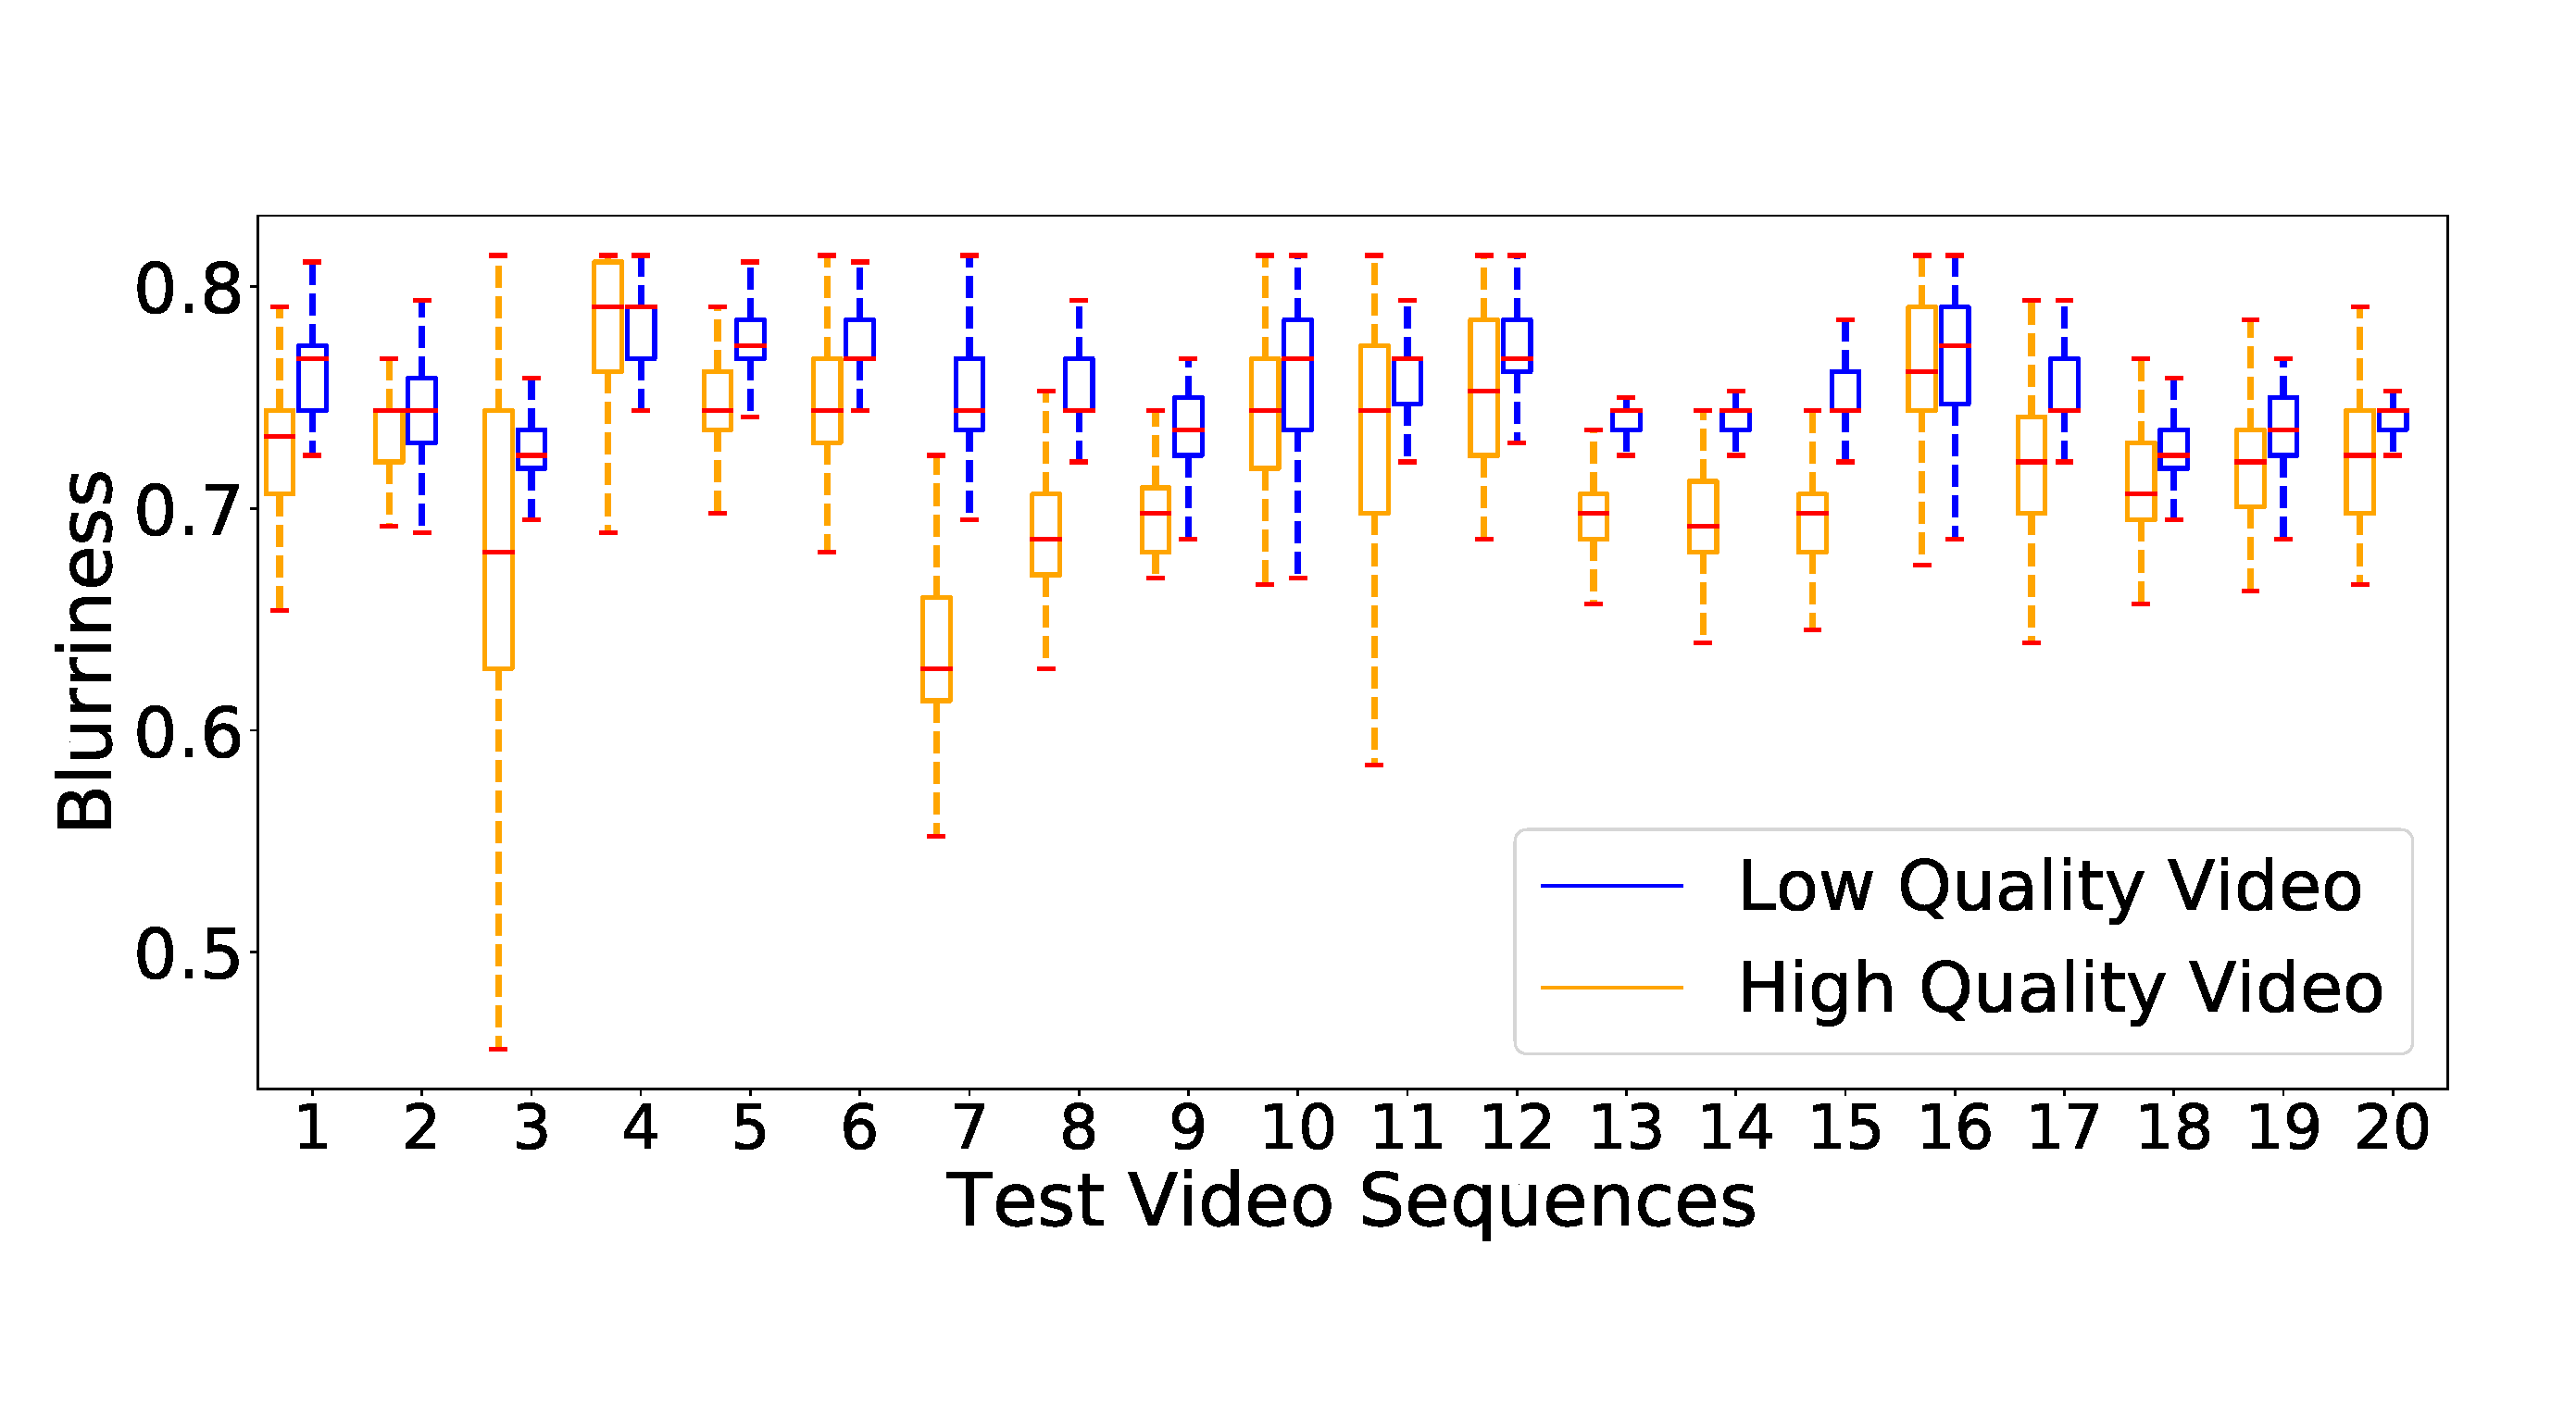
\includegraphics[width=0.45\textwidth]{sections/network-work/dct-blur}
	\vspace*{-2em}
	\caption{Blur detection using DCT coefficients~\cite{jana2016qoe,marichal1999blur}. DCT coefficients fail to distinguish between high and low quality video due to content diversity.}
	\label{fig:ucdavis}
	\vspace*{-0.5cm}
\end{figure}

We notice two aberrations of the DCT metric by Jana {\em et al}~\cite{jana2016qoe}: First, the metric is indeed content-specific i.e., although it produces high blur values for some low quality videos, it also shows high blur values for some high quality videos. For instance, videos 2 and 4 contain mostly over-illuminated and dark images and are equally tagged as blurred in both low and high quality scenarios. Second, DCT metric fails to detect accurate blur levels, even if the image is blurred heavily i.e., it shows low blur differences ($<$0.2 blurriness) between high and low quality videos even though we created extremely low-quality videos (240p resolution and high ($>$200\%) compression). Even for a single video, this DCT metric shows a lot of variation, such as for videos 3 and 11, raising concerns about its accuracy. We evaluate the accuracy of this blurriness metric in Section \ref{label:model}, showing a MOS error larger than 1.2. We also experiment with four other well-known blur metrics \cite{golestaneh2014no, mittal2012no, tong2004blur, marziliano2002no}, but none of these methods are consistent across diverse videos. This challenges the scalability and versatility of this blur metric in the wild. 

The {\em temporal variation} metric proposed by Jana {\em et al}~\cite{jana2016qoe} aims to capture video stalls and considers the ratio of missed frames to total number of frames in a video, but the metric requires the number of frames sent over the network. We need the reference video to compute the total number of frames in the video, thus the metric is not entirely no-reference. 
In enterprise networks, a QoE metric needs to be applicable to diverse contents and to not rely on access to reference video.
Further, there are many other previous works \cite{wolf2009no, borer2010model, usman2017no, pastrana2006automatic} focused on measuring the temporal jerkiness. We find these methods  either are parametrized or are sensitive to resolution and to frame rate of the video or are unable to scale across diverse video contents. The above limitations motivate us to propose new metrics that can accurately measure blurriness and freezes across diverse video content.

{\bf Need for a model per application category:}
When analyzing a recorded video for an application, the QoE metric has to be sensitive to the application category as different applications have to meet diverse performance guarantees. For instance, streaming quality is impacted largely by buffering and stall ratio, whereas telephony quality is impacted by bit rate, frames per second, blocking and blurring in the video. Table~\ref{tab:qoe_metric} lists examples of QoE metrics corresponding to different applications. Therefore, one needs to capture different artefacts when designing models for multiple application categories.

To address the aforementioned requirements, we seek to answer the question: {\em How to scalably label the quality of a video call, without any support from the application?}

\begin{table}[htb!]
	\centering
	\scriptsize
	\vspace*{-0.5em}	
%	\hspace{0.2in}
%	\parbox{.5\linewidth} {
		%\scalebox{1.1}{
            \resizebox{\columnwidth}{!}{
			\begin{tabular}{l|c}				
				\hline \hline
				\textbf{Application Category} & \textbf{Suitable Metric} \\
				\hline
				\hline
				Adaptive Streaming & Startup delay, Buffering ratio, Stall ratio \\ \hline
				Video Telephony & Bitrate, Fps, Blocking, Blurring \\ \hline
				Progressive Downloads & PSNR, SSIM \\ \hline
				VR/AR, Game Streaming & Latency, buffering ratio, Stall ratio \\ \hline 
			\end{tabular}
		}
	\vspace*{0.5em}
		\hfill 
		\caption{Metrics based on application category}
		\label{tab:qoe_metric}
%	}
	\vspace*{-1em}
\end{table}

